\documentclass[10pt,letterpaper,conference,onecolumn]{ieeeconf}
\IEEEoverridecommandlockouts
\overrideIEEEmargins
\usepackage[T1]{fontenc}
\usepackage{amsmath,amssymb,graphicx,booktabs,url}
\makeatletter
\setlength{\@fptop}{0pt}
\setlength{\@fpsep}{12pt}
\setlength{\@fpbot}{0pt plus 1fil}
\makeatother
\newtheorem{proposition}{Proposition}
\newcommand{\norm}[1]{\left\lVert#1\right\rVert}
\title{Supplementary Diagnostics and Evidence Index\\Boundary Deployment and Contact Feasibility\\in Cooperative Transport without Prior Object Geometry}
\author{Development manuscript --- author information pending}
\date{4 November 2026}
\begin{document}
\maketitle
This supplement preserves additional mathematical diagnostics and measured trajectories. It does not add simulated episodes or extend the claims of the eight-page main manuscript. The batches below have distinct source identities and cannot be pooled as independent repetitions. The result registry is \texttt{RESULTS\_INDEX.md}; current validation records are in \texttt{docs/results/resource\_noise\_validation\_v1/} from the repository root.

\section{Restricted feedback diagnostics}
% Retained mathematical and signed-error diagnostics from the earlier main text.
\subsection{Restricted information analysis}
For fixed point-to-plane correspondences and small pure translation,
\begin{equation}
b=A\Delta x+\epsilon,\qquad j=d^T\Delta x.
\end{equation}
\begin{proposition}
The noiseless task scalar is identifiable for every displacement iff
$d\in\operatorname{range}(A^T)$. When identifiable, minimum-norm exact weights are
$\ell=A(A^TA)^\dagger d$, and
$|\ell^Tb-j|\leq\norm{\ell}\norm{\epsilon}$.
\end{proposition}
\noindent\emph{Proof:} Indistinguishable translations differ by $z\in\ker A$; their task scalars agree iff $d^Tz=0$ for every such $z$. Exact weights satisfy $A^T\ell=d$; the minimum-norm solution is as stated, and Cauchy--Schwarz gives the bound.\hfill$\square$

This standard fact excludes uncertain normals, incorrect association, rotation and evolving maps. A circle's absolute rotation ambiguity does not imply that its translation is unidentifiable. Polygon discretization is part of our executed model. The earlier synthetic observation-layout test is preserved as supplementary diagnosis; no new sensing policy is evaluated in the census.

The rejected candidate reads
\begin{equation}
\widehat J^{a}_k=g\bigl(d^Tm_k^-+\ell_k^Tb_k\bigr),\qquad g=1.24.
\end{equation}
It retains the historical map anchor. Under the restrictive rigid-map residual model
$b_k=A_k[(x_k-x_0)-m_k^-]+\eta_k$,
its error is $(g-1)J_k+g\ell_k^T\eta_k$.
A correct certificate does not remove the gain term or bound real map/correspondence errors. This equation is a limitation, not evidence that gain alone caused the observed failures.

\subsection{Signed cumulative accounting from existing logs}
The offline audit uses the recorded pre-physics control-time truth. For robot $i$, define $u_{ik}=d^Tm^+_{ik}$, held-readout term
$h_{ik}=r^{\rm original}_{ik}-gu_{ik}$, and candidate term
$c_{ik}=r_{ik}-r^{\rm original}_{ik}$. Then
$r_{ik}=u_{ik}+(g-1)u_{ik}+h_{ik}+c_{ik}$.
Median weights $w_{ik}$ reproduce actual team progress $T_k$; tied values use an explicit agent-ID rule. The component allocation is not unique at ties and is not a causal attribution.

With $E_k=T_k-J_k$,
\begin{align}
\Delta E_k={}&\sum_iw_{ik}(\Delta u_{ik}-\Delta J_k)
+\sum_iw_{ik}(g-1)\Delta u_{ik}\nonumber\\
&+\sum_iw_{ik}\Delta h_{ik}+\sum_iw_{ik}\Delta c_{ik}
+\sum_i\Delta w_{ik}r_{i,k-1}.
\end{align}
Accumulating all terms and the initial error reconstructs the signed error; omitting the voter-change term would misallocate it. Registration plus fusion also reconstructs map increments to numerical precision. Both are accounting checks, not physical-estimation proofs.

\begin{table}[t]
\caption{Baseline cumulative signed-error accounting, millimeters, at the last aligned control instant. Components use a fixed median tie rule and are not causal effects. Displayed terms are rounded.}
\centering\footnotesize
\begin{tabular}{lrrrrr}\toprule
Case & Map--truth & Gain & Held & Voters & Total\\\midrule
R2 & -18.9 & 306.0 & -13.9 & -102.4 & 170.8 \\
L8 & -168.7 & 236.4 & 36.6 & 50.7 & 154.9 \\
C8 & -240.0 & 255.7 & 22.5 & -2.1 & 36.0 \\
\bottomrule\end{tabular}
\end{table}
The residual of cumulative reconstruction is below $10^{-12}$ m in every arm. The different signed terms can compensate or reinforce each other; they do not isolate an implementation defect. The raw-map, gain, hold and endogenous voter effects remain hypotheses for future targeted tests, not a reason to tune this completed batch.


For the v2 baseline episodes, the first shared HOLD in rectangle and L occurs with true speeds zero but endpoint errors outside the original task tolerance. Estimated/true progress is $1.4651/1.2939$ m against $L=1.4467$ m for rectangle, and $1.3082/1.1535$ m against $L=1.3044$ m for L. C has already reached the projected goal. These observations identify premature spatial stopping in the selected failures. Individual transport-loop hysteretic holding states were not saved; their exact first transitions cannot be reconstructed from scalar input alone. No new gain, certificate or candidate is introduced.


\begin{figure*}[t]
\centering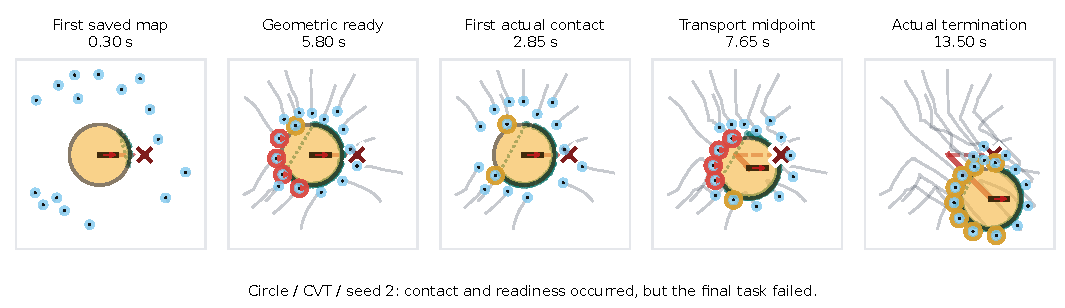
\includegraphics[width=\textwidth]{generated/media_v1/full_process.pdf}
\caption{Circle/CVT event-indexed process: first saved local map, geometric readiness, first physical contact, transport midpoint and actual termination. Event columns need not be chronological: contact here precedes readiness. Orange is evaluation geometry, teal is agent 00's fused map, and rings mark geometric readiness, not contact. The final task fails despite G500 passing.}
\label{fig:process}
\end{figure*}

\clearpage
\section{Historical complete-task comparison}
The nine-condition, seed-2 census changes the deployment module while retaining the common downstream implementation. All 27 cases are displayed. This historical source/configuration is separate from the 2026-11-04 validation. Boundary CVT and spacing each spatially complete five of nine tasks; nearest completes two. Failed runs have actual termination times, not successful completion times. Command-path length is not physical energy.
\begin{figure}[!ht]
\centering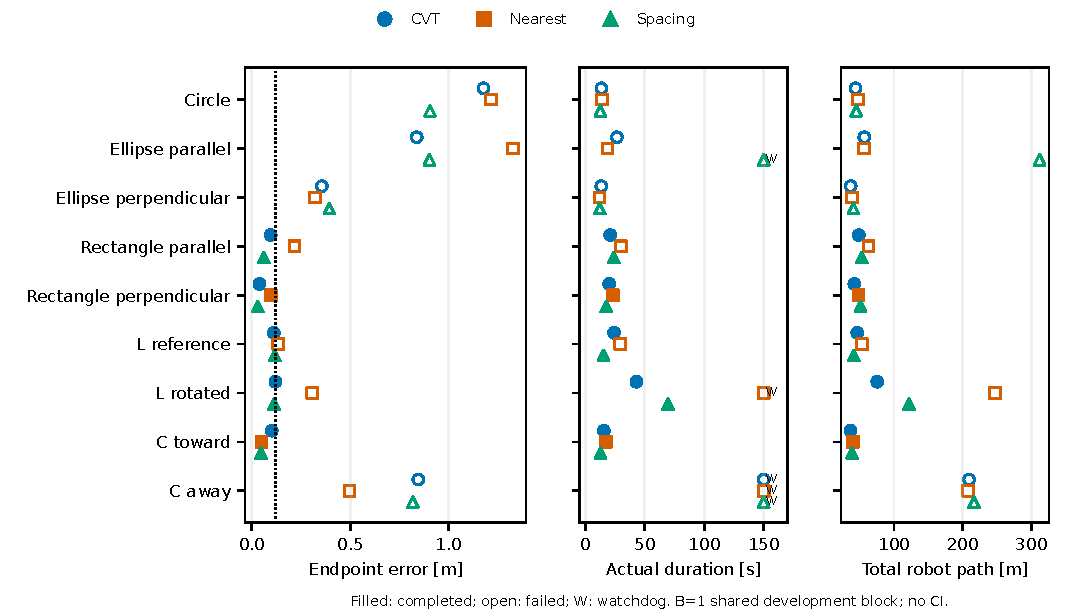
\includegraphics[width=\textwidth]{generated/media_v1/method_comparison.pdf}
\caption{All 27 census tasks: complete denominator, endpoint error, actual duration and robot path. Filled/open markers denote spatial completion/failure. W marks a watchdog. One shared random scene block; no inferential confidence intervals.}
\end{figure}
\begin{figure}[!ht]
\centering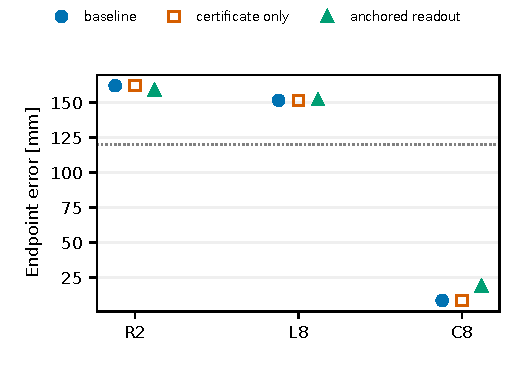
\includegraphics[width=.5\textwidth]{generated/media_v1/v2_negative.pdf}
\caption{Separate rejected feedback candidate. The passive certificate reproduces the original execution; anchored feedback rescues neither selected failure and worsens C8. These are selected development cases, not independent generalization evidence.}
\end{figure}

\clearpage
\section{Current-source five-shape stages}
\begin{figure}[!ht]
\centering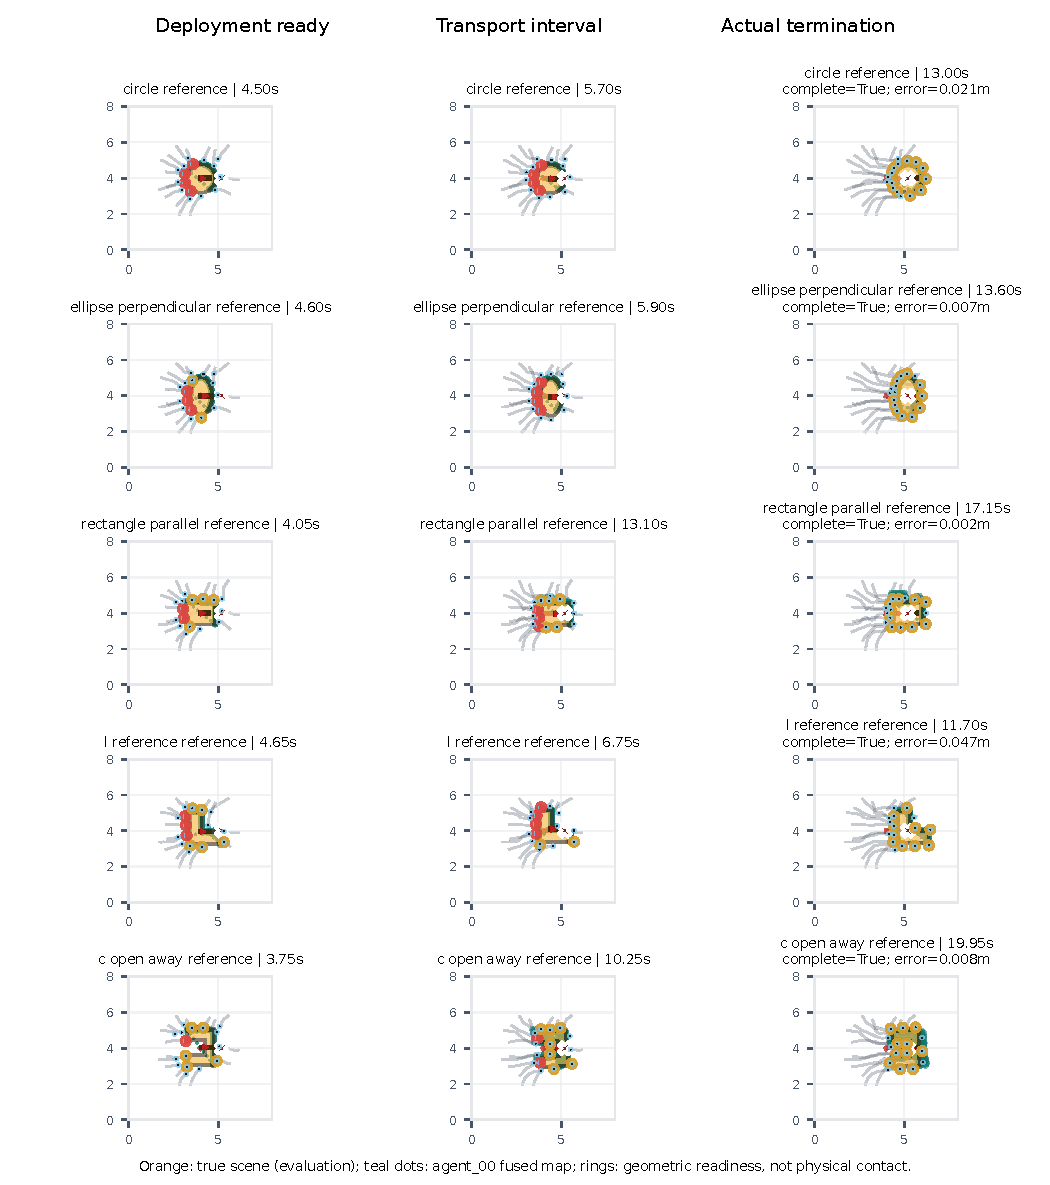
\includegraphics[width=.95\textwidth,height=.77\textheight,keepaspectratio]{generated/resource_noise/five_shape_stages.pdf}
\caption{Five prospectively selected CVT reference conditions, seed 2026110401, 16 robots and range noise $\sigma=0.01$ m. Columns show the measured state immediately after the first geometric readiness event, a midpoint in the transport interval, and the actual terminal state. Event names do not certify physical contact or completion. All five displayed reference cases complete; failures in the other regimes remain in the complete table and subsequent diagnostics. Orange is offline evaluation geometry, teal is agent 00's fused map, and rings show geometric readiness. No raw laser rays or unrecorded motion are inferred.}
\end{figure}

\clearpage
\section{Current vector navigation and stopping}
\begin{figure}[!ht]
\centering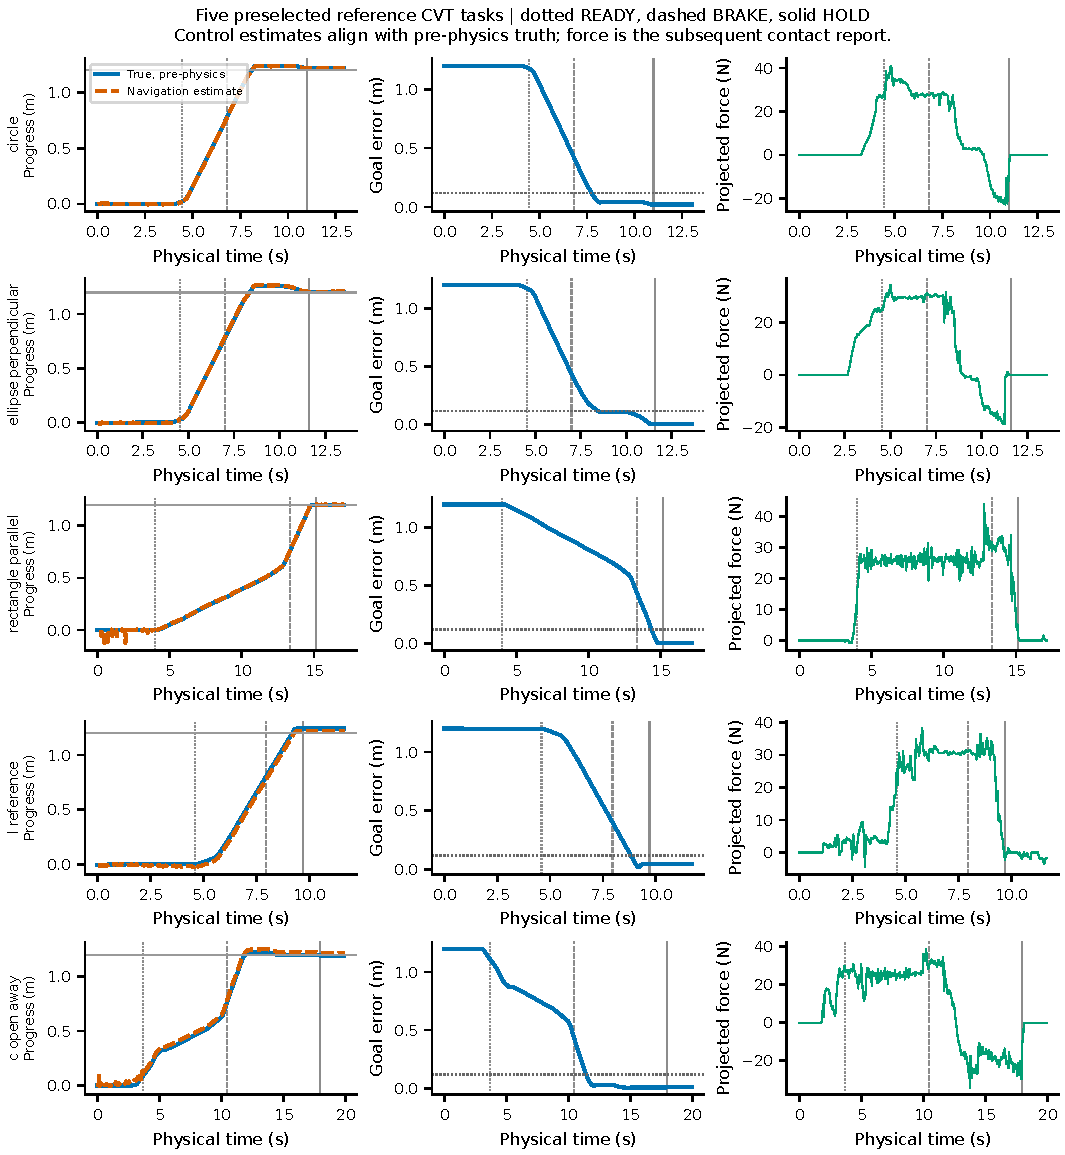
\includegraphics[width=\textwidth,height=.83\textheight,keepaspectratio]{generated/resource_noise/reference_navigation.pdf}
\caption{All five preselected reference CVT trajectories. Navigation estimates are the recorded shared vector-displacement readout projected onto the task direction, compared with pre-physics truth. The auxiliary scalar feedback shown in replay media is not substituted for this navigation signal. Goal error uses actual trace poses; contact force belongs to the subsequent contact calculation in each step. READY, BRAKE and HOLD are recorded supervisor events, with no imputed event. All control samples are retained without smoothing.}
\end{figure}

\clearpage
\section{Current resource failures and evidence boundaries}
The C-away, eight-robot condition was selected after the validation to inspect both incomplete trajectories and their matched CVT control. No new physical trajectory or parameter change is introduced. CVT eventually satisfies spatial completion at 571.55 s. Spacing ends at 600 s in BRAKE with 0.110190 m endpoint error, which is inside the positional tolerance but does not satisfy the HOLD dwell. Nearest reaches HOLD at 46.65 s and terminates at 48.65 s, 0.823656 m from the goal. Recorded motion and stopping can occur without the TRANSPORT activation event; the monotone supervisor may skip intermediate phases. These observations identify distinct contract failures, not a unique causal estimator fault.
\begin{figure}[!ht]
\centering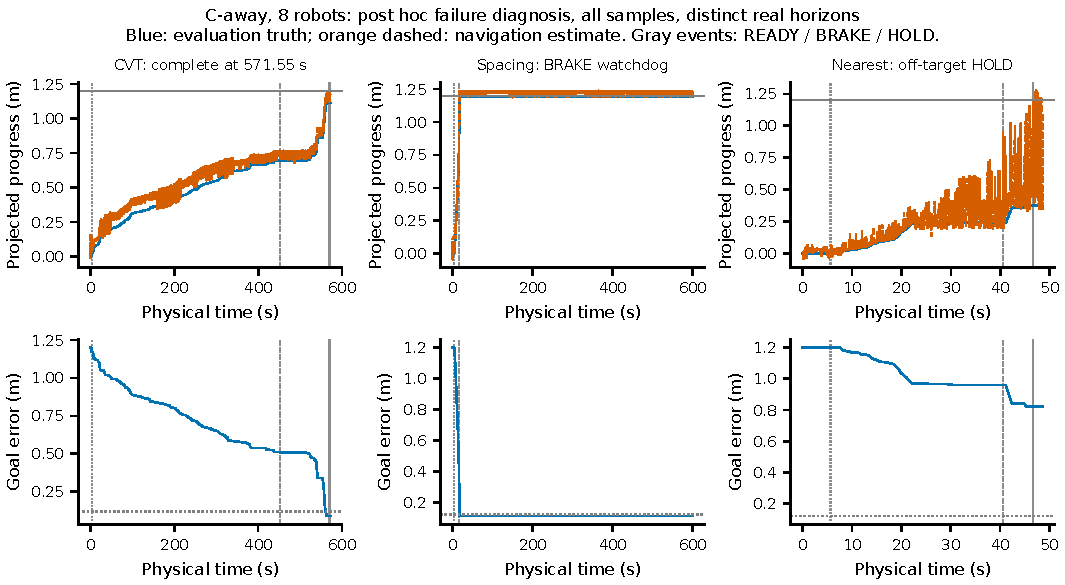
\includegraphics[width=\textwidth]{generated/resource_noise/c8_failure_diagnostics.pdf}
\caption{Post hoc diagnosis of all three matched C-away/eight-robot cases, with their distinct measured time horizons. True projected displacement, shared navigation estimate and two-dimensional endpoint error are separate quantities. Gray event lines retain actual READY/BRAKE/HOLD decisions; spacing has no HOLD. The companion synchronized MP4 retains the whole 600 s horizon at 1 s sampling and $10\times$ playback. Ended cases hold their real final state.}
\end{figure}

Increasing the team to 24 robots also exposes two original hard-safety failures. L/CVT reaches maximum penetration 0.120428 m against its 0.0975 m discrete budget; ellipse-perpendicular/spacing reaches 0.115719 m against 0.1002 m. Both spatially complete but are excluded from completion without hard safety failure. No post hoc change to the penetration allowance or settling rule is made. These safety measurements concern the penalty/contact simulator and discrete evaluator, not certified continuous separation or hardware behavior.

The finite-support branch in the main paper remains rejected. Its interrupted full-trajectory constraint audit is quarantined as incomplete; the eight physical outcomes and fixed 336-system optimization witnesses are separately identified. Conditional local-polygon admission requires an occupancy enclosure and motion bound that have not been implemented. Neither design text nor a numerical witness substitutes for an end-to-end safety or transport theorem.

\section{Reproducibility and workflow}
All Python work uses the root project environment. The fresh regression records report 1113 passed and two skipped core tests, and 106 passed MAS-platform tests. An earlier sandbox temporary-directory failure is preserved separately. The scientific runtime and protected configuration remain unchanged; presentation and audit helpers do not establish new algorithm behavior. AI assistance and pending author review are disclosed in the package README.

The current workload benchmark used one, four and eight processes on the same eight 100-step engineering prefixes, and selected eight after exact replay comparison. Timings are 92.374, 34.126 and 22.108 s including startup. The 60 scientific cases took 779.104 s. A one-prefix profile is not a whole-run optimization claim; engineering prefixes are excluded from scientific denominators. Matplotlib produces source-bound vector figures, FFmpeg encodes and fully decodes the videos, and Inkscape 1.4.4 verifies a vector export. No GPU acceleration of the physical solver is claimed.

\end{document}
